%% This is file `elsarticle-template-1-num.tex',
%%
%% Copyright 2009 Elsevier Ltd
%%
%% This file is part of the 'Elsarticle Bundle'.
%% ---------------------------------------------
%%
%% It may be distributed under the conditions of the LaTeX Project Public
%% License, either version 1.2 of this license or (at your option) any
%% later version.  The latest version of this license is in
%%    http://www.latex-project.org/lppl.txt
%% and version 1.2 or later is part of all distributions of LaTeX
%% version 1999/12/01 or later.
%%
%% The list of all files belonging to the 'Elsarticle Bundle' is
%% given in the file `manifest.txt'.
%%
%% Template article for Elsevier's document class `elsarticle'
%% with numbered style bibliographic references
%%
%% $Id: elsarticle-template-1-num.tex 149 2009-10-08 05:01:15Z rishi $
%% $URL: http://lenova.river-valley.com/svn/elsbst/trunk/elsarticle-template-1-num.tex $
%%
\documentclass[preprint,12pt]{elsarticle}



%% Use the option review to obtain double line spacing
%% \documentclass[preprint,review,12pt]{elsarticle}

%% Use the options 1p,twocolumn; 3p; 3p,twocolumn; 5p; or 5p,twocolumn
%% for a journal layout:
%% \documentclass[final,1p,times]{elsarticle}
%% \documentclass[final,1p,times,twocolumn]{elsarticle}
%% \documentclass[final,3p,times]{elsarticle}
%% \documentclass[final,3p,times,twocolumn]{elsarticle}
%% \documentclass[final,5p,times]{elsarticle}
%% \documentclass[final,5p,times,twocolumn]{elsarticle}

%% if you use PostScript figures in your article
%% use the graphics package for simple commands
%% \usepackage{graphics}
%% or use the graphicx package for more complicated commands
%% \usepackage{graphicx}
%% or use the epsfig package if you prefer to use the old commands
%% \usepackage{epsfig}

%% The amssymb package provides various useful mathematical symbols
\usepackage{amssymb}
%% The amsthm package provides extended theorem environments
%% \usepackage{amsthm}

%% The lineno packages adds line numbers. Start line numbering with
%% \begin{linenumbers}, end it with \end{linenumbers}. Or switch it on
%% for the whole article with \linenumbers after \end{frontmatter}.
\usepackage{lineno}
\usepackage{hyperref}
\usepackage{quoting}
\usepackage{float}
\usepackage{lipsum}
\usepackage{tikz}
\usepackage{minted}
\usetikzlibrary{matrix,shapes,arrows,positioning,chains}

% load package with some of the available options - you may not need this!
\usepackage[autolinebreaks,useliterate]{mcode}



%% natbib.sty is loaded by default. However, natbib options can be
%% provided with \biboptions{...} command. Following options are
%% valid:

%%   round  -  round parentheses are used (default)
%%   square -  square brackets are used   [option]
%%   curly  -  curly braces are used      {option}
%%   angle  -  angle brackets are used    <option>
%%   semicolon  -  multiple citations separated by semi-colon
%%   colon  - same as semicolon, an earlier confusion
%%   comma  -  separated by comma
%%   numbers-  selects numerical citations
%%   super  -  numerical citations as superscripts
%%   sort   -  sorts multiple citations according to order in ref. list
%%   sort&compress   -  like sort, but also compresses numerical citations
%%   compress - compresses without sorting
%%
%% \biboptions{comma,round}

% \biboptions{}

\begin{document}
	
	\tikzset{
		desicion/.style={
			diamond,
			draw,
			text width=3em,
			text badly centered,
			inner sep=0pt
		},
		block/.style={
			rectangle,
			draw,
			text width=18em,
			text centered,
			rounded corners
		},
		cloud/.style={
			draw,
			ellipse,
			minimum height=2em
		},
		descr/.style={
			fill=white,
			inner sep=2.5pt
		},
		connector/.style={
			-latex,
			font=\scriptsize
		},
		rectangle connector/.style={
			connector,
			to path={(\tikztostart) -- ++(#1,0pt) \tikztonodes |- (\tikztotarget) },
			pos=0.5
		},
		rectangle connector/.default=-2cm,
		straight connector/.style={
			connector,
			to path=--(\tikztotarget) \tikztonodes
		}
	}

\begin{frontmatter}

%% Title, authors and addresses

%% use the tnoteref command within \title for footnotes;
%% use the tnotetext command for the associated footnote;
%% use the fnref command within \author or \address for footnotes;
%% use the fntext command for the associated footnote;
%% use the corref command within \author for corresponding author footnotes;
%% use the cortext command for the associated footnote;
%% use the ead command for the email address,
%% and the form \ead[url] for the home page:
%%
%% \title{Title\tnoteref{label1}}
%% \tnotetext[label1]{}
%% \author{Name\corref{cor1}\fnref{label2}}
%% \ead{email address}
%% \ead[url]{home page}
%% \fntext[label2]{}
%% \cortext[cor1]{}
%% \address{Address\fnref{label3}}
%% \fntext[label3]{}

\title{Confronto implementazioni Metodo di Cholesky\\
\large{Attraverso l'utilizzo di ambienti differenti: Matlab, C++ e R}
\vspace{5mm}\\ \normalsize{\texttt{https://github.com/nicoripa/MCS\_Project/}}}
%% use optional labels to link authors explicitly to addresses:
%% \author[label1,label2]{<author name>}
%% \address[label1]{<address>}
%% \address[label2]{<address>}

\author{Lorenzo Rovida, Nicolò Ripamonti\\
	\small{ \href{mailto:l.rovida1@campus.unimib.it}{l.rovida1@campus.unimib.it},  \href{mailto:n.ripamonti@campus.unimib.it}{n.ripamonti@campus.unimib.it}\\817151, 816171}}

\address{Dipartimento di Informatica, Sistemi e Comunicazione, Universitá degli Studi di Milano-Bicocca, Milano, Italia}


\begin{abstract}
Lo scopo di questo progetto è di studiare l'implementazione in ambienti di programmazione open source del metodo di \textbf{Cholesky} per la risoluzione sistemi lineari per matrici sparse, simmetriche e definite positive e successivamente confrontarli con l’implementazione nell'ambiente di programmazione di Matlab.
	
Immaginiamo che un'azienda abbia la necessità di munirsi di un ambiente di programmazione per risolvere sistemi lineari con matrici sparse e definite positive di grandi dimensioni utilizzando il metodo di Cholesky. 
	
L'alternativa è tra software proprietario (Matlab) oppure open source e anche tra Windows oppure Linux.
	
La richiesta è quindi quella di confrontare, in ambiente Linux e Windows, e sulla stessa macchina, l'ambiente di programmazione Matlab con una libreria open source. 
	
In altre parole bisogna porsi le seguenti domande:
\begin{enumerate}
		\item \`E meglio lavorare in ambiente Linux oppure in ambiente Windows?
		
		\item \`E meglio affidarsi alla sicurezza di Matlab pagando oppure vale la pena di avventurarsi nel mondo open source? 
		
\end{enumerate}
\end{abstract}
	


\end{frontmatter}

%%
%% Start line numbering here if you want
%%

%% main text
\newpage

\section{Introduzione}

Lo scopo di questo progetto è quello di valutare l’implementazione, in ambienti di programmazione differenti, del metodo di Cholesky per la risoluzione di sistemi lineari per matrici sparse. La scelta degli ambienti, da parte del team, si è focalizzata su:

\begin{center}
	\textbf{Matlab} \quad - \quad \textbf{C++} \quad - \quad \textbf{R}
\end{center}

Le matrici che sono state considerate per la realizzazione del progetto sono quelle del gruppo \textit{SuiteSparse Matrix Collection} che colleziona matrici sparse derivanti da applicazioni di problemi reali (ingegneria strutturale, fluidodinamica, elettromagnetismo, termodinamica, computer graphics/vision, network e grafi).

In particolare le matrici simmetriche e definite positive che sono state analizzate sono le seguenti:
\begin{center}
	\begin{itemize}
		\item \textbf{Flan\_1565}
		\item \textbf{StocF-1465}
		\item \textbf{cfd2}
		\item \textbf{cfd1}
		\item \textbf{G3\_circuit}
		\item \textbf{parabolic\_fem}
		\item \textbf{apache2}
		\item \textbf{shallow\_water1}
		\item \textbf{ex15}
	\end{itemize}
	
\end{center}

Un sistema lineare si può rappresentare in forma matriciale come $ A \cdot x = b $
dove:
\begin{itemize}
	\item A è la matrice dei coefficienti del sistema ed è rappresentata da una delle matrici del gruppo \textit{SuiteSparse Matrix Collection} elencate precedentemente.
	\item x è il vettore colonna delle incognite.
	\item b è il vettore colonna dei termini noti; b è scelto in modo che la soluzione esatta sia il vettore $ xe = [1 1 1 \dots 1 1] $ avente tutte le componenti uguali a 1, tale che $ b = A \cdot xe $ .
\end{itemize}


\subsection{Matrici sparse}
Le matrici sparse sono una classe di matrici con la caratteristica di contenere un significativo numero di elementi uguali a zero. Spesso il numero di elementi diversi da zero su ogni riga è un numero piccolo (per esempio del- l’ordine di $10^1$) indipendente dalla dimensione della matrice, che può essere anche dell’ordine di $10^8$.

Le matrici sparse si possono memorizzare in modo compatto, tenendo solo conto degli elementi diversi da zero; per esempio, è sufficiente per ogni elemento diverso da zero memorizzare solo la sua posizione $i j$ e il suo valore $a_{ij}$, ignorando gli elementi uguali a zero. Ciò consente di ridurre il tempo di calcolo eliminando operazioni su elementi nulli.

\subsection{Calcolatore utilizzato}

Per effettare i diversi calcoli è stato utilizzato un Surface Book 2 con le seguenti caratteristiche hardware:
\begin{itemize}
	\item Intel Core i5-7300U @ 2.60GHz 2.71GHz
	\item CPU x64
	\item 8.00 GB RAM
	\item Intel HD Graphics 620
\end{itemize}

Il sistema operativo installato e utilizzato per Matlab, C++ e R è stato Windows 10, successivamente è stato incluso nel confronto lo stesso codice C++ lanciato su Ubuntu 20.04 LTS installato su WSL (Windows Subsystem Linux).

In dettaglio sono stati utilizzati:
\begin{itemize}
	\item MATLAB R2020a
	\item g++ (i686-posix-dwarf-rev0, Built by MinGW-W64 project) 8.1.0 (Ambiente Windows)
	\item RStudio (basato su R versione 3.6.2)
	\item g++ (Ubuntu 9.3.0-10ubuntu2) 9.3.0 (Ambiente Ubuntu)
\end{itemize}

\newpage


\section{Ambienti di sviluppo}

Il confronto dei vari ambienti di programmazione sui sistemi operativi di Windows e Linux deve avvenire in termini di:
\begin{description}
	\item[Tempo:] Calcolo dei tempi di esecuzione del metodo di Cholesky;
	\item[Accuratezza:] Calcolo dell'errore assoluto tra la soluzione esatta e la soluzione del sistema lineare;
	\item[Impiego della memoria:] Quantità di memoria utilizzata per il calcolo del sistema lineare con il metodo di Cholesky.
\end{description}


\subsection{Matlab}
\medskip
\begin{description}
	\item[Versione:] 9.7.0
	\item[Referenze:] \href{https://it.mathworks.com/products/matlab.html}{Sito} - \href{https://www.mathworks.com/help/matlab/}{Documentazione}
\end{description}

Matlab (abbreviazione di Matrix Laboratory) è un ambiente per il calcolo numerico e l'analisi statistica scritto in C, che comprende anche l'omonimo linguaggio di programmazione creato dalla MathWorks. MATLAB consente di manipolare matrici, visualizzare funzioni e dati, implementare algoritmi, creare interfacce utente, e interfacciarsi con altri programmi. Matlab è usato da milioni di persone nell'industria e nelle università per via dei suoi numerosi strumenti a supporto dei più disparati campi di studio applicati e funziona su diversi sistemi operativi, tra cui Windows, Mac OS, GNU/Linux e Unix.

\subsection{Eigen, C++}
\medskip
\begin{description}
	\item[Versione:] 3.7.7, Novembre 2019
	\item[Referenze:] \href{http://eigen.tuxfamily.org/index.php?title=Main_Page}{Sito} - \href{http://eigen.tuxfamily.org/dox/}{Documentazione}
\end{description}

\textit{Eigen} è una libreria di modelli C++ per l'algebra lineare, ovvero che supporta il calcolo e la risoluzione di matrici, vettori, solutori numerici e algoritmi correlati.

Supporta matrici di qualsiasi dimensione, dalle piccole matrici di dimensioni fisse alle matrici dense arbitrariamente grandi, fino alle matrici sparse e il suo ecosistema offre molte funzionalità specializzate come l'ottimizzazione non lineare, le funzioni di matrice, un solutore polinomiale e molto altro.

\textit{"L'implementazione di un algoritmo su Eigen è come copiare semplicemente lo pseudocodice."}

Eigen ha un buon supporto per il compilatore mentre si esegue una suite di test per garantire affidabilità e aggirare eventuali bug del compilatore. Eigen è anche standard C ++ 98 e mantiene tempi di compilazione molto ragionevoli.

Eigen è un software open source concesso in licenza con Mozilla Public License 2.0 dalla versione 3.1.1.

In particolare di Eigen sono state utilizzate le funzioni:
\begin{description}
	\item[\texttt{SimplicialLDLT}] Questa classe fornisce fattorizzazioni $LDL^ T$ Cholesky di matrici sparse che sono definite positive. La fattorizzazione consente di risolvere $AX = B$ dove $X$ e $B$ possono essere densi o sparsi. Al fine di ridurre il riempimento, viene applicata una permutazione simmetrica $P$ prima della fattorizzazione in modo tale che la matrice fattorizzata sia $PAP ^ {-1}$;
	\item[\texttt{solve()}] Funzione utilizzata per trovare la soluzione di x.
\end{description}


\subsection{Matrix, R}
\medskip
\begin{description}
	\item[Versione:] 1.2-18, Novembre 2018
	\item[Referenze:] \href{http://matrix.r-forge.r-project.org}{Sito} - \href{https://www.rdocumentation.org/packages/Matrix}{Documentazione}
\end{description}

Il pacchetto di R \textit{Matrix} fornisce un set di classi per matrici dense e sparse che estendono le classi base delle matrici già presenti in R. I metodi per un'ampia gamma di funzioni e operatori applicati agli oggetti di queste classi forniscono un accesso efficiente alla soluzione di sistemi lineari, matrici dense e matrici sparse.

Una caratteristica notevole del pacchetto è che ogni volta che una matrice viene fattorizzata, la fattorizzazione viene memorizzata come parte della matrice originale in modo che ulteriori operazioni sulla matrice possano riutilizzare questa fattorizzazione.

In particolare del pacchetto Matrix, sono state usate due funzioni:

\begin{description}
	\item[\texttt{readMM()}] Funzione utilizzata per leggere un file di tipo MatrixMarket. All'interno della funzione basta inserire il percorso del file;
	\item[\texttt{chol()}] Funzione che calcola la fattorizzazione di Choleski di una matrice quadrata simmetrica e definita positiva. Gli argomenti che si possono inserire all'interno della funzione sono:
	\begin{description}
		\item[x] Una matrice quadrata (sparsa o densa); se x non è definito positivo, viene segnalato un errore. per la nostra implementazione abbiamo utilizzato come argomento della funzione solamente la matrice;
		\item[pivot] Valore logico che indica se si deve usare il pivot. Attualmente, questo non viene utilizzato per matrici dense.
		\item[cache] Valore logico che indica se il risultato deve essere memorizzato nella cache; si noti che questo argomento è sperimentale e disponibile solo per alcune matrici sparse.
	\end{description}
\end{description}

\newpage


\section{Implementazioni}

L'implementazione del metodo è stata così suddivisa:

\begin{center}


\begin{tikzpicture}
\matrix (m)[matrix of nodes, column  sep=3cm,row  sep=10mm, align=center, nodes={rectangle,draw, anchor=center} ]{
	|[block]| {Start}       \\
	|[block]| {\textbf{Setup} \\ Caricamento matrice in \textit{A}, creazione soluzione \textit{xe}, calcolo $b = A \times xe$.}     \\
	|[block]| {\textbf{Cholesky} \\ Calcolo della matrice di Cholesky \textit{R}.}     \\
	|[block]| {\textbf{Soluzione} \\ Calcolo soluzione del sistema sfruttando l'ipotesi di Cholesky $A = R \times R'$}     \\
	|[block]| {Calcolo dell'errore relativo di \textit{x} rispetto a \textit{xe}}     \\
	|[block]| {\textbf{Fine}}    \\
};
\path [>=latex,->] (m-1-1) edge (m-2-1);
\path [>=latex,->] (m-2-1) edge (m-3-1);
\path [>=latex,->] (m-3-1) edge (m-4-1);
\path [>=latex,->] (m-4-1) edge (m-5-1);
\path [>=latex,->] (m-5-1) edge (m-6-1);

\end{tikzpicture}

\end{center}

Le fasi segnate in grassetto verranno cronometrate dal sistema, da notare come l'ultima parte (il calcolo dell'errore) non venga inclusa nella misurazione, essa infatti non farà parte di un ipotetico codice definitivo (una volta scelto il linguaggio non non sarà più necessario calcolare l'errore e tantomeno cronometrare le funzioni).

\newpage

\subsection{Matlab}
L'implementazione su ambiente Matlab è stata effettuata tramite questo semplice script:

\begin{lstlisting}
tic

%Leggo la matrice A
A = Problem.A;

%Creo soluzione che e' un vettore lungo righe di A con tutti 1
xe = ones(size(A,1), 1);

%Calcolo b dalla equazione A * xe = b
b = A * xe;

disp('Time setup:');
toc
tic

%Calcolo Cholesky triangolare inferiore della matrice A 
R = chol(A);

disp('Time Cholesky:');
toc
tic

%{
Siccome per ipotesi di Cholesky A = R * R',
allora risolvere Ax = b diventa R * R' * x = b,
quindi x = R \ (R' \ b)
%}

y = R' \ b;
x = R \ y;

disp('Time resolve:');
toc

%Calcolo errore fra x e xe
errore = norm(x - xe) / norm(xe);

disp('Errore: ');
disp(errore);

\end{lstlisting}

da notare l'utilizzo dei comandi \mcode{tic} e \mcode{toc}, utili per visualizzare il tempo utile per il calcolo di determinati blocchi di codice.
\linebreak


\textit{Pro e contro - Script Matlab}\\
\vspace{4mm}
L'implementazione di Matlab può essere riassunta con questi pro e contro:

Pro:
\begin{itemize}
	\item Codice compatto e intuitivo
	\item Interfaccia user friendly con gestione variabili e console
\end{itemize}

Contro:
\begin{itemize}
	\item Closed source
\end{itemize}

\newpage

\subsection{R}

La soluzione per ambiente R è data dal seguente script:

\begin{figure}[H]
	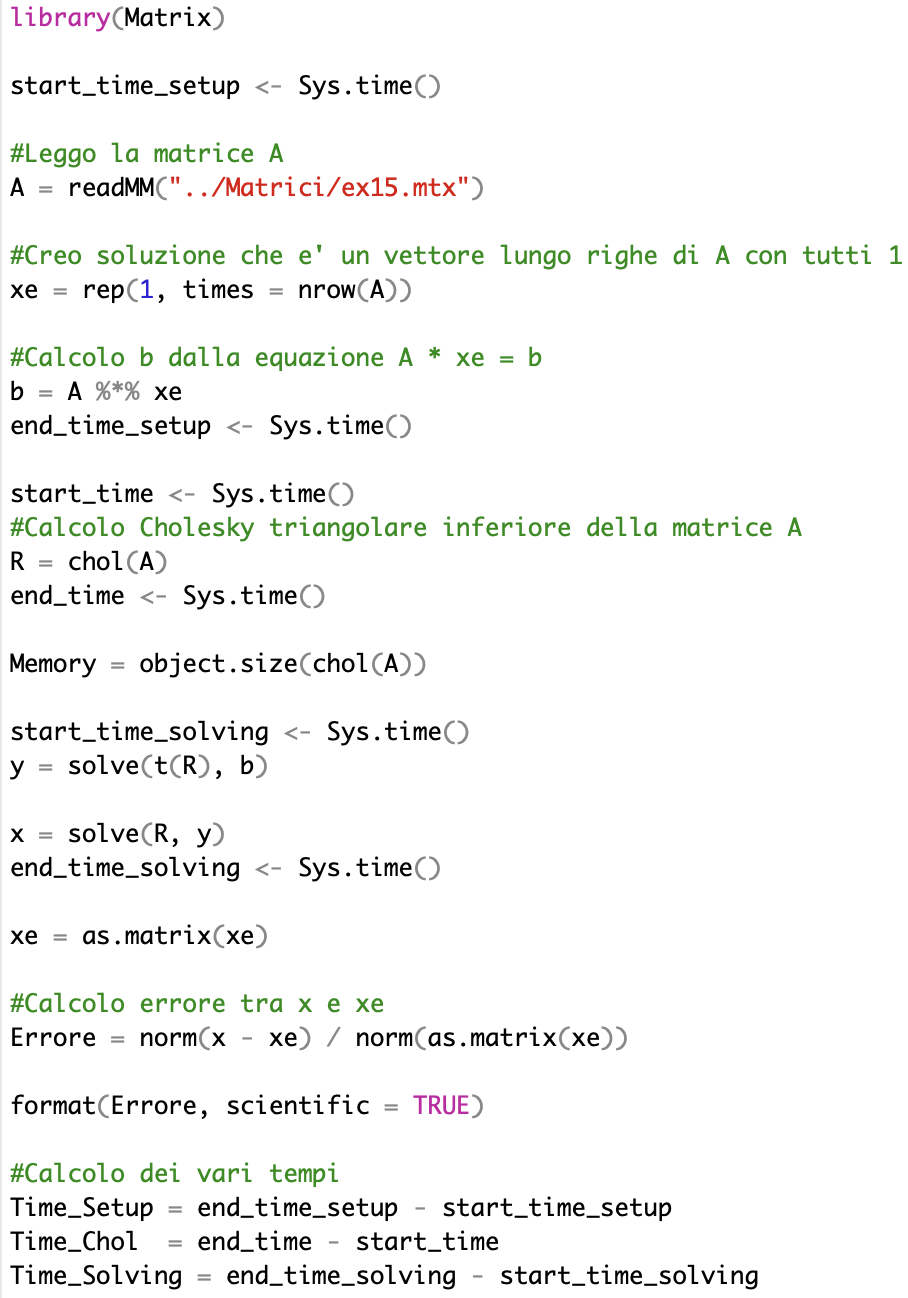
\includegraphics[width=0.80\textwidth]{rcode}
\end{figure}

Una differenza sostanziale con il codice Matlab è data dalla presenza di una variabile che contiene la memoria utilizzata. Tale funzione è stata molto utile per calcolare la memoria utilizzata dallo script (per gli altri ambienti abbiamo utilizzato tool del sistema operativo per tener monitorato l'utilizzo della memoria).
\medskip


\textit{Pro e contro - Script R}\\
\vspace{4mm}
L'implementazione di R può essere riassunta con questi pro e contro:

Pro:
\begin{itemize}
	\item Interfaccia user friendly con gestione variabili e console
	\item Supportato da diverse librerie open-source facili da includere
\end{itemize}

Contro:
\begin{itemize}
	\item Sintassi troppo "flessibile" (non ci sono regole precise da seguire)
\end{itemize}

\newpage

\subsection{C++}

Il file \textit{script.cpp} è costruito sul seguente codice:

\begin{minted}{c}
#include <iostream>
#include <Eigen/Dense>
#include <unsupported/Eigen/SparseExtra>
#include <Eigen/SparseCholesky>
#include <chrono>

using namespace std;
using namespace Eigen;
using namespace chrono;

int main(int argc, char** argv) {	

  cout << endl;

  for (int i = 1; i < argc; ++i) {

    cout << "Cholesky con " << argv[i] << endl;		
    
    steady_clock::time_point begin = steady_clock::now();

    SparseMatrix<double> A;

    loadMarket(A, argv[i]);

    VectorXd xe = VectorXd::Constant(A.rows(), 1);

    VectorXd b = A.selfadjointView<Lower>() * xe;

    steady_clock::time_point end = steady_clock::now();

    cout << "Time Setup = " 
         << duration_cast<nanoseconds>(end - begin).count() 
         << "ns" << endl;
         
    begin = steady_clock::now();

    SimplicialLDLT<SparseMatrix<double>> chol(A);

    end = steady_clock::now();
    
    cout << "Time Cholesky = " 
         << duration_cast<nanoseconds>(end - begin).count()
         << "ns" << endl;
         
    begin = steady_clock::now();

    VectorXd x = chol.solve(b);
    
    end = steady_clock::now();

  
    cout << "Time Resolve = " 
         << duration_cast<nanoseconds>(end - begin).count() 
         << "ns" << endl;

    double relative_error = (x - xe).norm() / (xe).norm();

    cout << "Relative error = " << relative_error << endl;

    cout << endl << "****" << endl << endl;
  }
}
\end{minted}

Come specificato in precedenza, questo script verrà lanciato sia su Windows che su WSL Ubuntu 20.04.
\medskip


\textit{Pro e contro - Script C++}\\
\vspace{4mm}
L'implementazione di C++ può essere riassunta con questi pro e contro:

Pro:
\begin{itemize}
	\item Moltissime librerie offrono supporto per qualsivoglia azione
	\item Velocità - C++ è un linguaggio compilato (a differenza dei linguaggi interpretati)
\end{itemize}

Contro:
\begin{itemize}
	\item Complicato da imparare, codice non facilmente leggibile
	\item Assenza di un'interfaccia per la gestione delle variabili ecc.
\end{itemize}

\newpage


\section{Elaborazioni e risultati}

Nella sezione corrente verranno presentati i risultati delle varie elaborazioni su grafici. Essi conterranno valori per matrici fino a 715.176 righe (\textit{apache2.mtx}) in quanto per matrici più grandi il calcolatore non riesce a portare a termine l'elaborazione (per mancanza di memoria).

\subsection{Time setup}La prima parte dell'analisi ha riguardato il tempo di setup, come specificato all'inizio della sezione 3.
In breve \textit{Time setup} è il tempo che intercorre tra il caricamento della matrice $A$, l'inizializzazione di $xe$ e il calcolo di $b$

\begin{figure}[H]
	\centering
	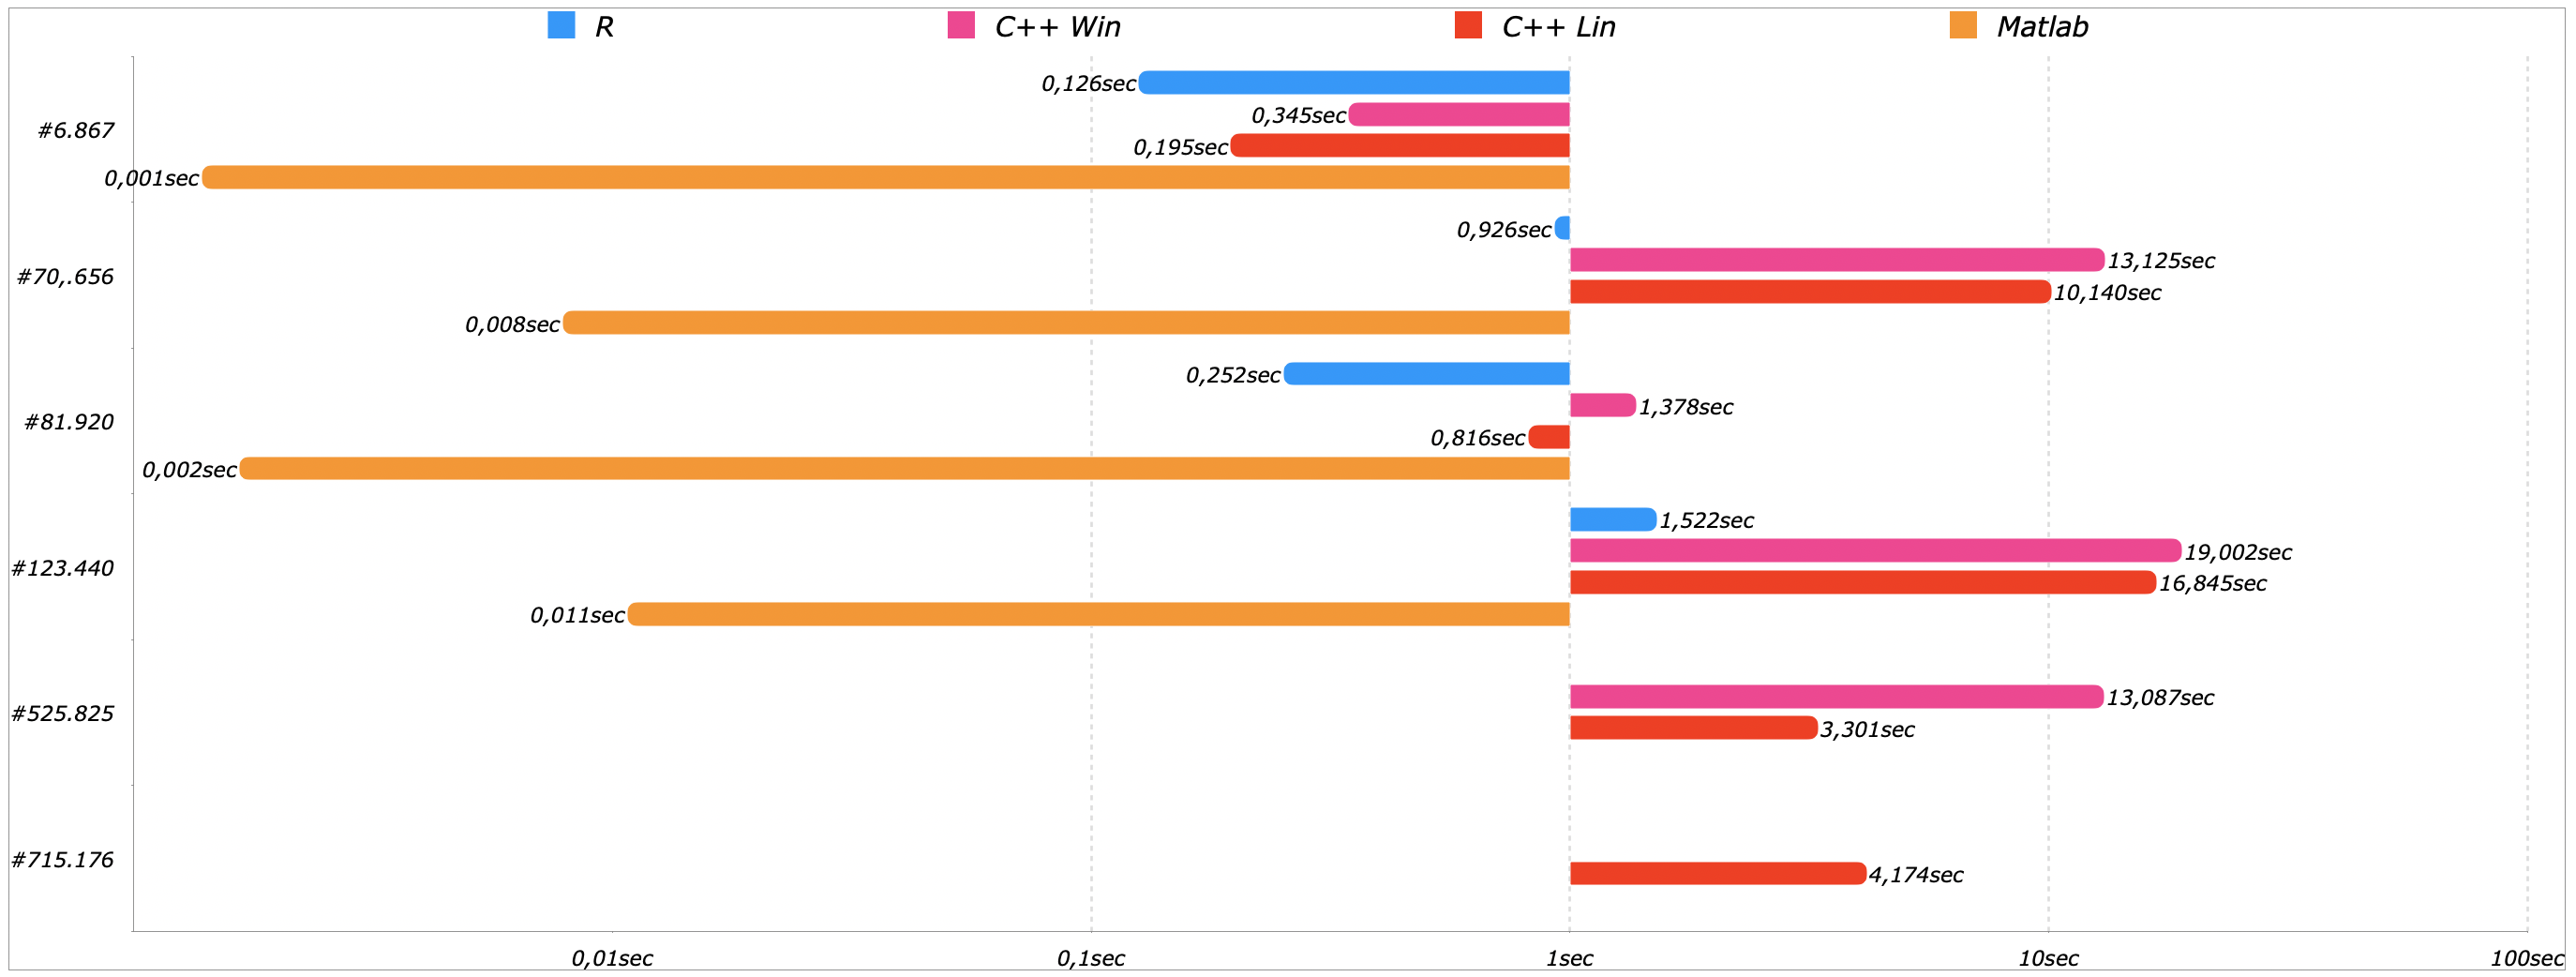
\includegraphics[width=\linewidth]{setup1}
\end{figure}

\begin{figure}[H]
	\centering
	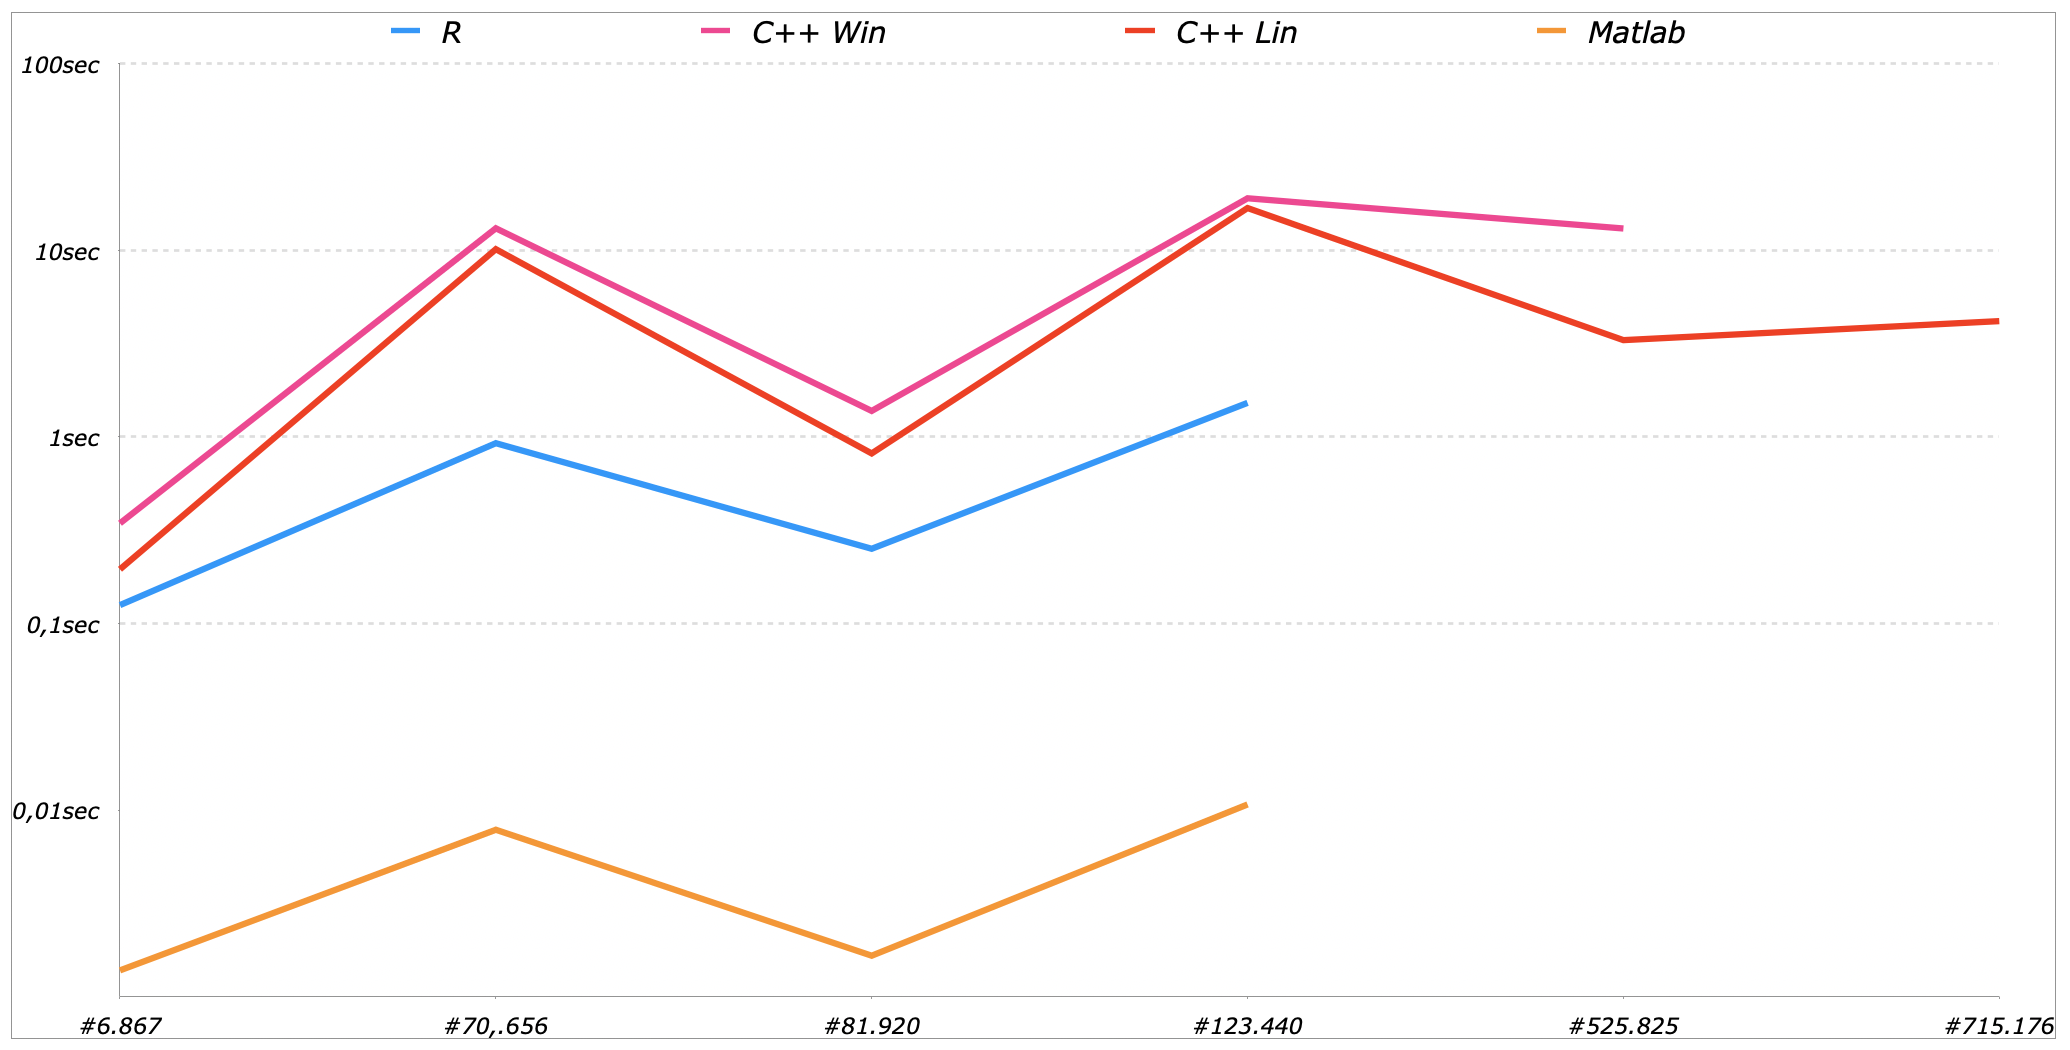
\includegraphics[width=\linewidth]{setup2}
\end{figure}

Come si può facilmente osservare chi impiega il minor tempo è Matlab, a seguire (molto distanti) rispettivamente R, C++ su Win e C++ su Linux.


Da notare però come Matlab ed R non riescano a gestire matrici con numero di righe $\geq 525.825$, cosa che C++ riesce a fare. Addirittura su ambiente linux il sistema riesce anche a gestire la matrice \textit{apache2.mtx} di dimensione 715.176.

\subsection{Time Cholesky}

\begin{figure}[H]
	\centering
	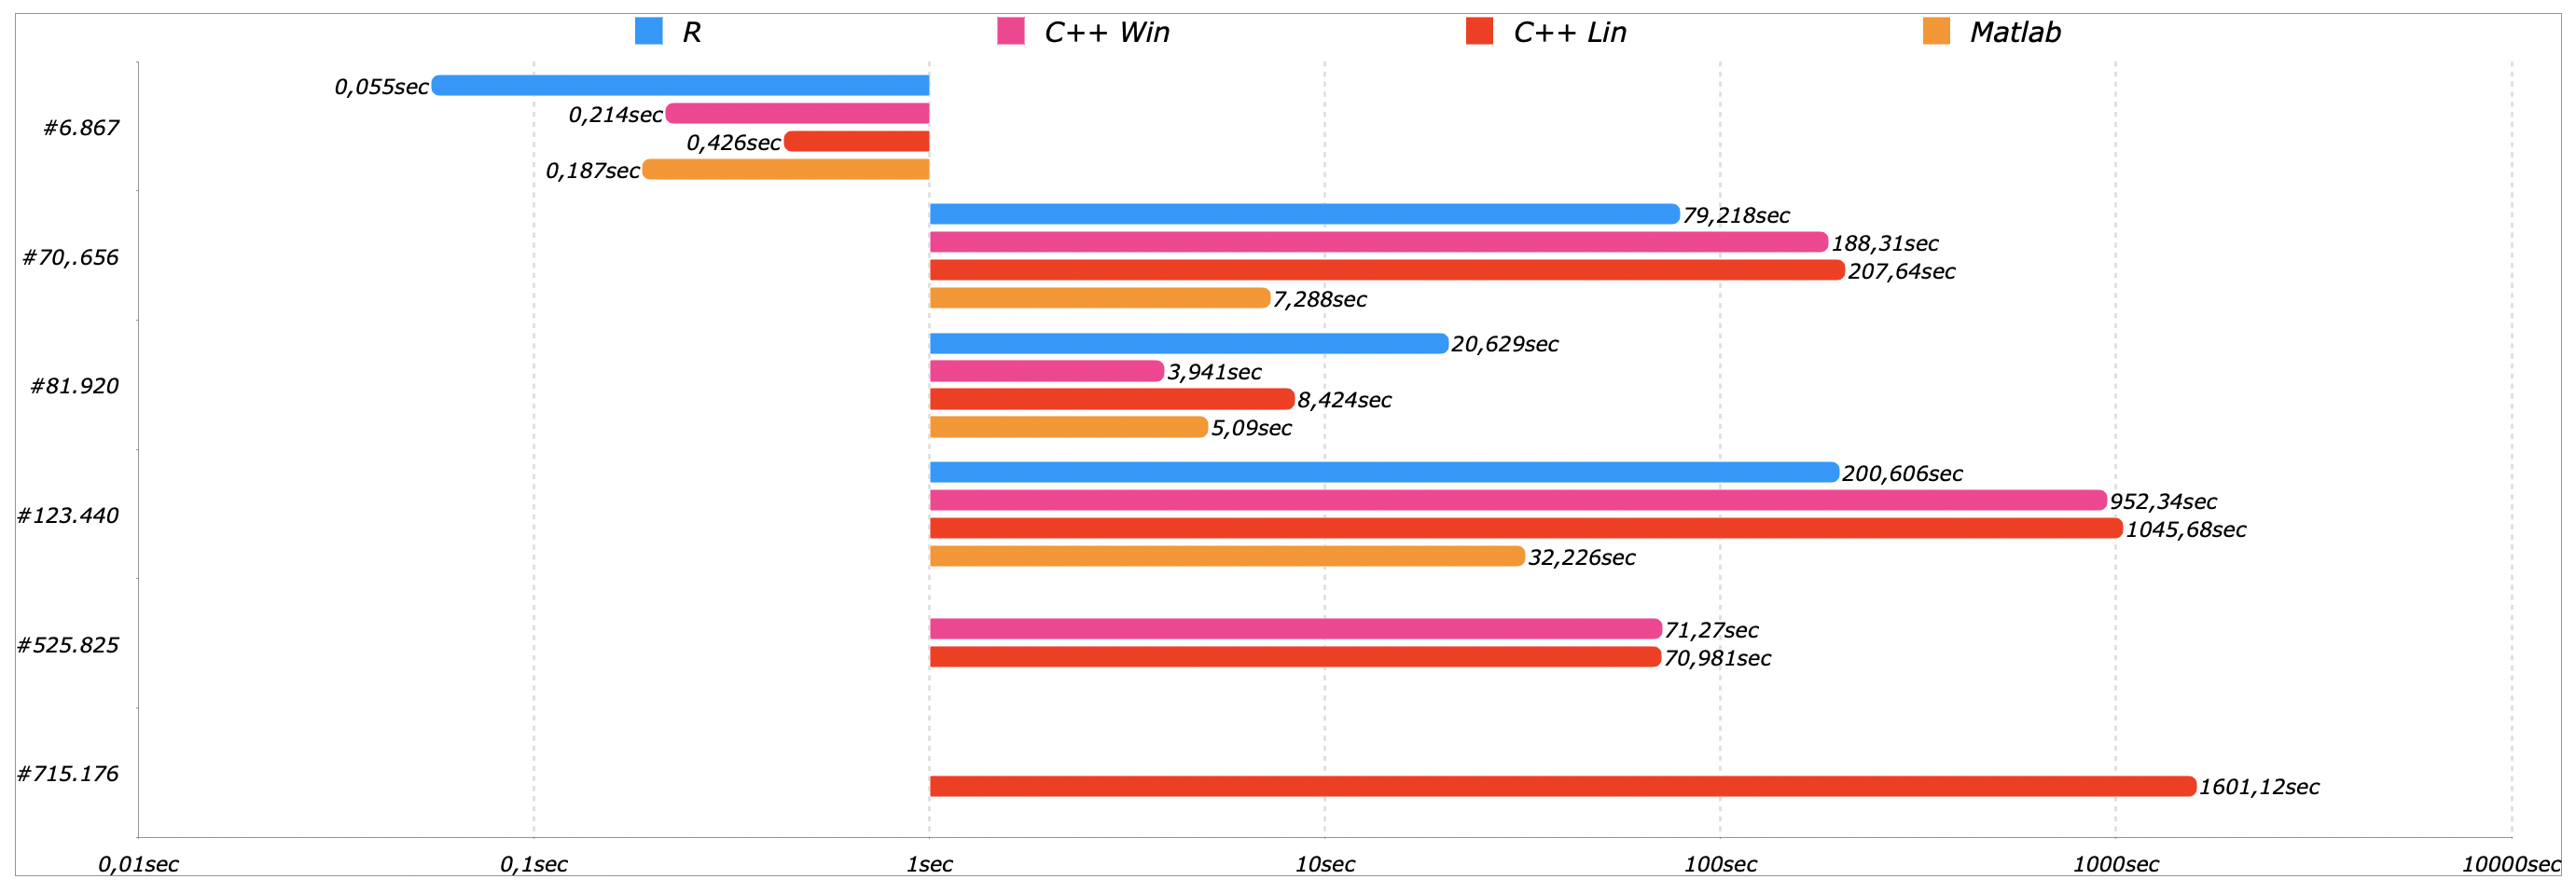
\includegraphics[width=\linewidth]{cholesky1}
\end{figure}

\begin{figure}[H]
	\centering
	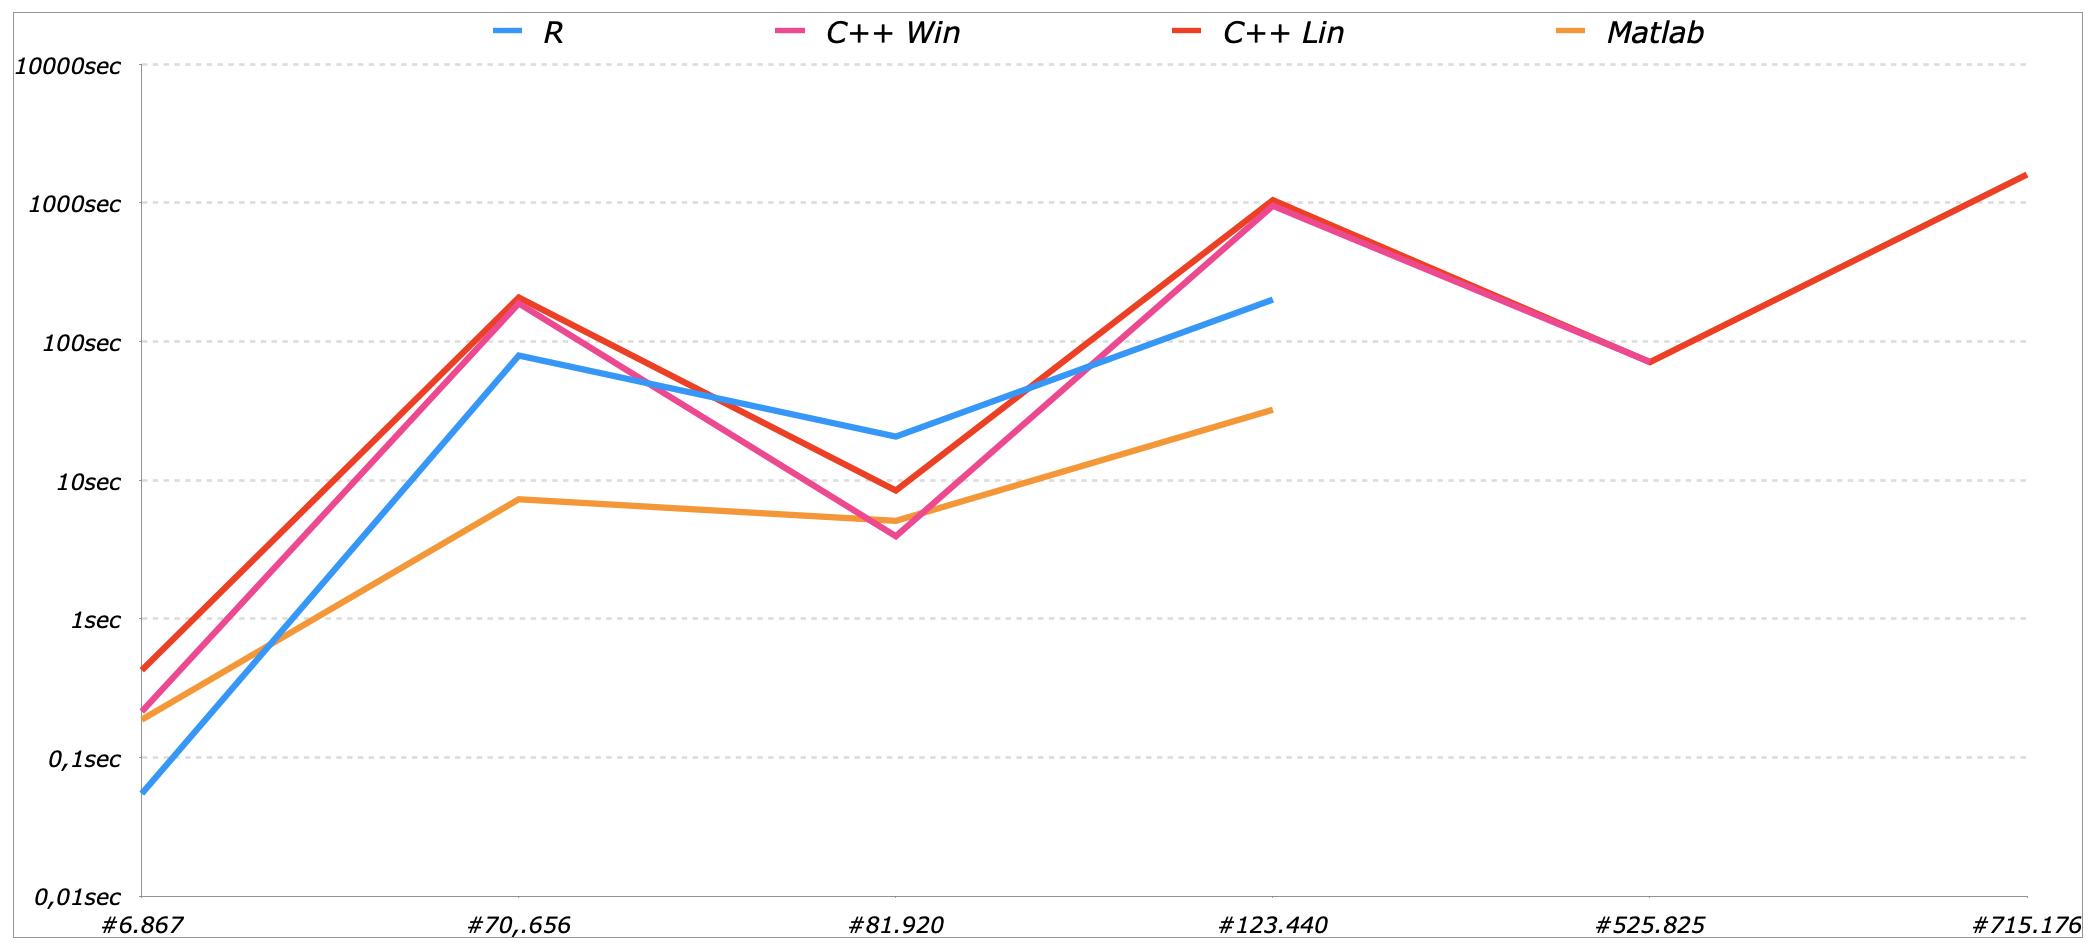
\includegraphics[width=\linewidth]{cholesky2}
\end{figure}

Questi grafici rappresentano il tempo forse più significativo, ovvero il tempo per il calcolo della matrice di Cholesky $R$.
Matlab si conferma l'ambiente tendenzialmente più rapido, anche se la differenza non sembra essere così significativa (nonostante ci sia).

\subsection{Time resolve}

\begin{figure}[H]
	\centering
	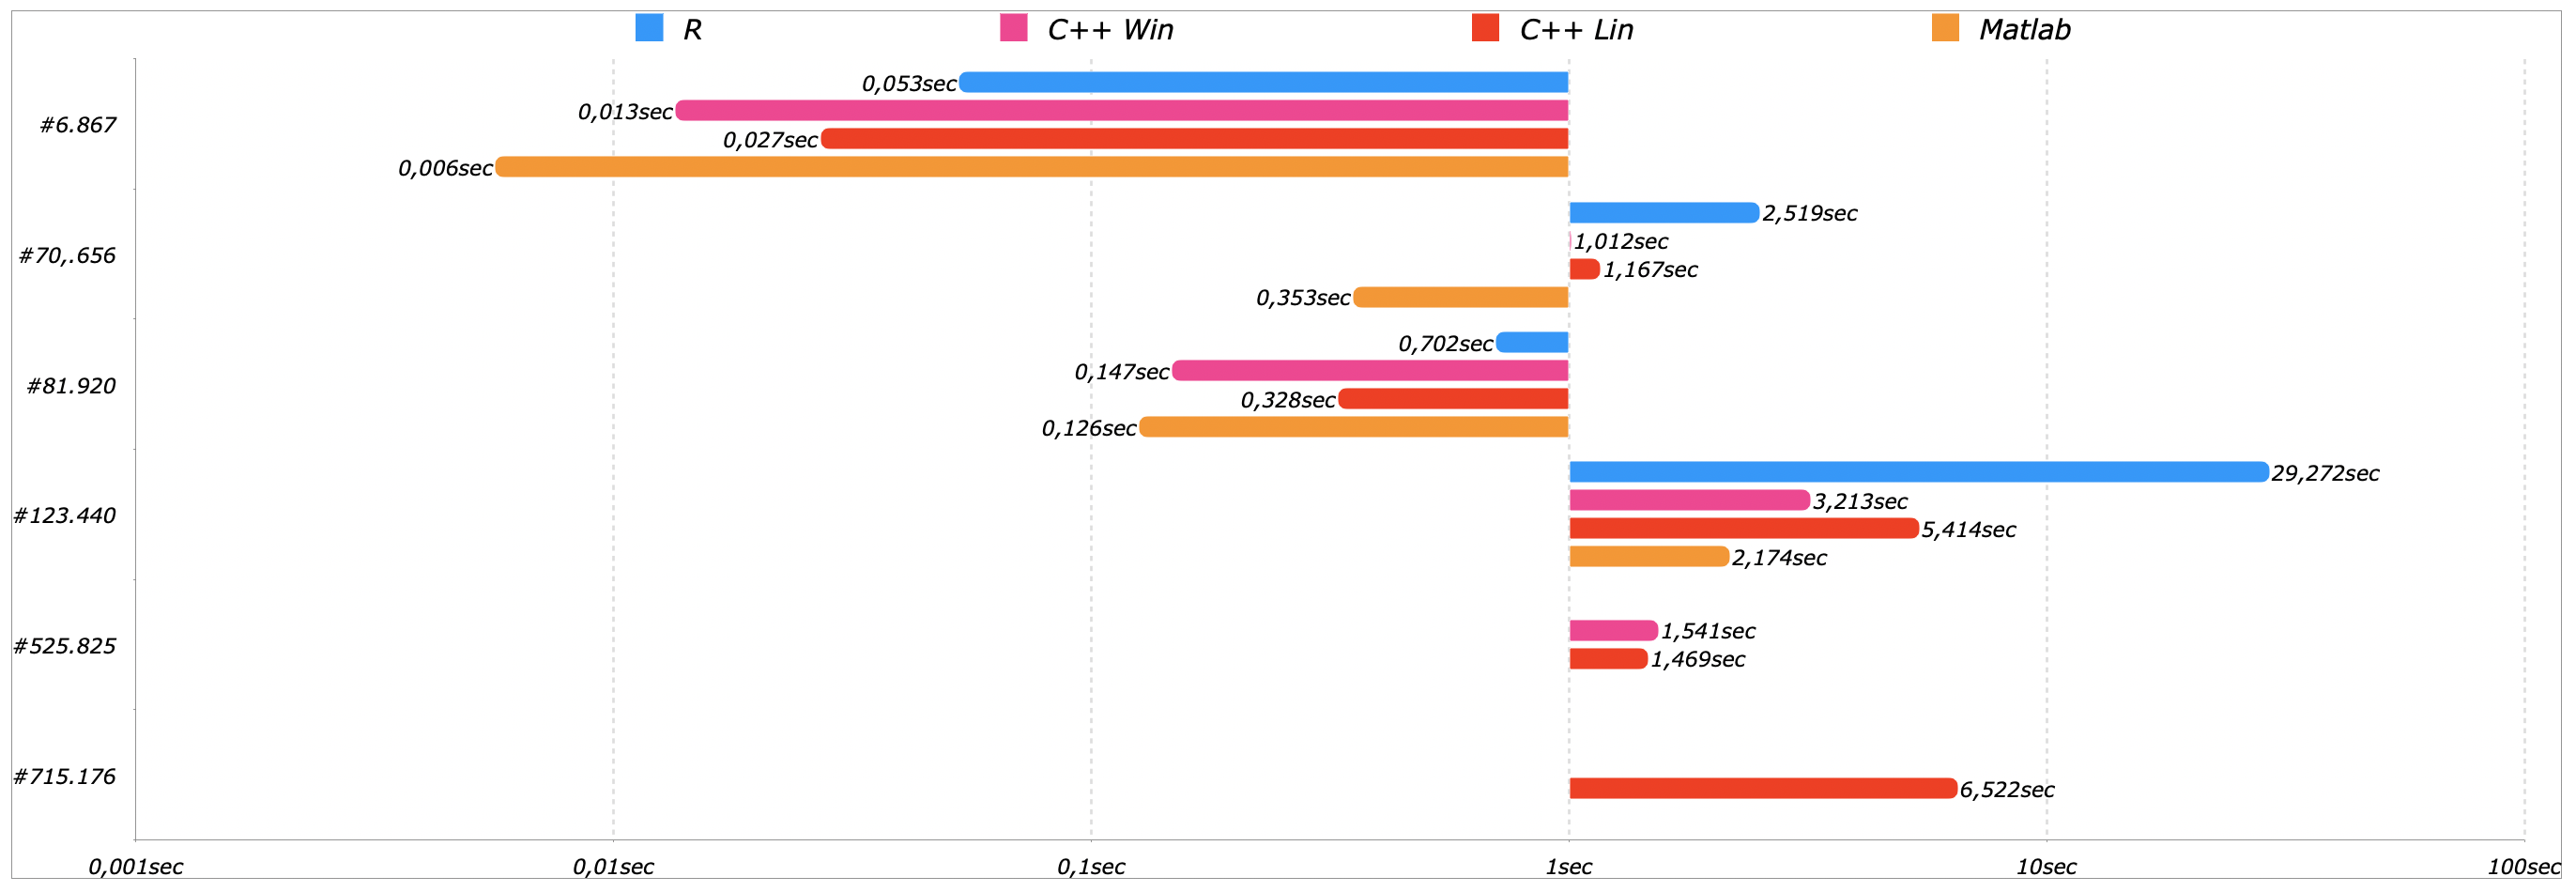
\includegraphics[width=\linewidth]{solving1}
\end{figure}

\begin{figure}[H]
	\centering
	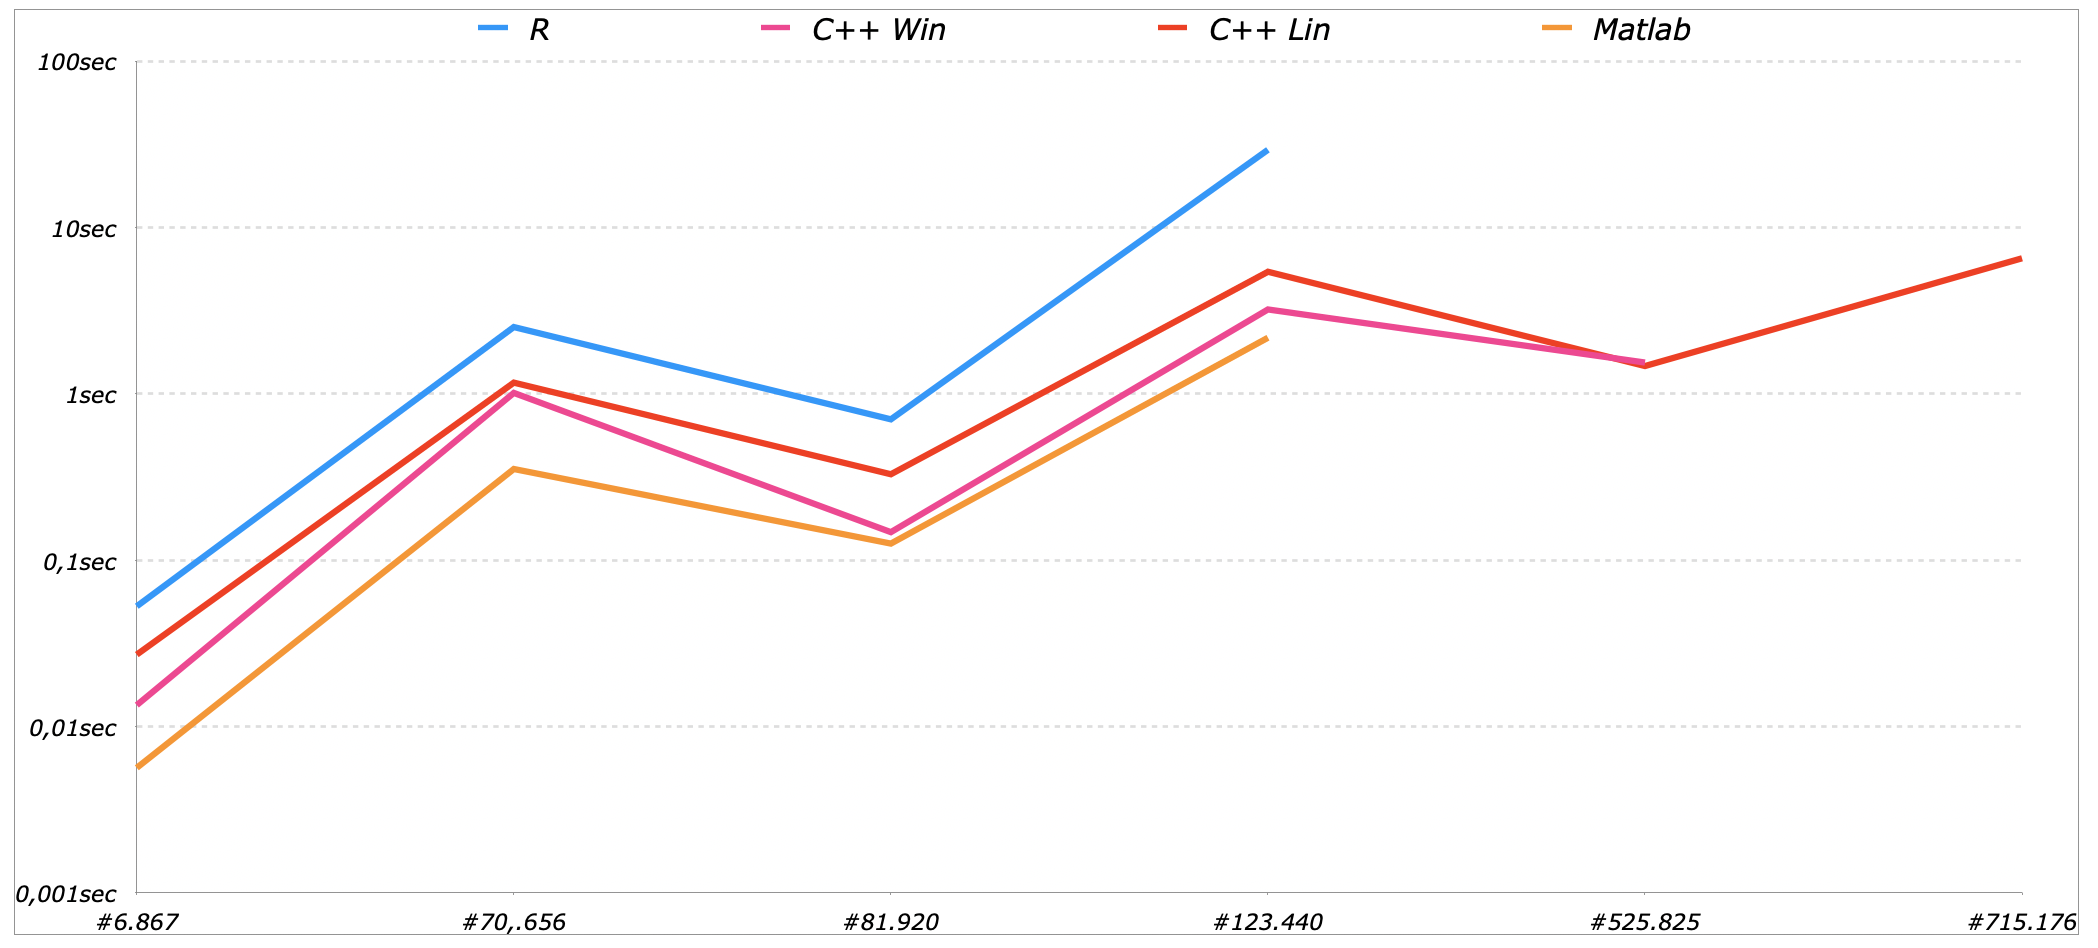
\includegraphics[width=\linewidth]{solving2}
\end{figure}

Questi grafici rappresentano il tempo impiegato per la risoluzione del sistema finale $R \times R' \times x = b$.
Come si può notare i vari linguaggi sembrano avere un comportamento molto simile, e anche qui si osserva la leggera superiorità di Matlab rispetto ai suoi concorrenti, mentre R si denota come il più lento, con dei tempi più lunghi rispetto agli altri.

\subsection{Errori relativi}

\begin{figure}[H]
	\centering
	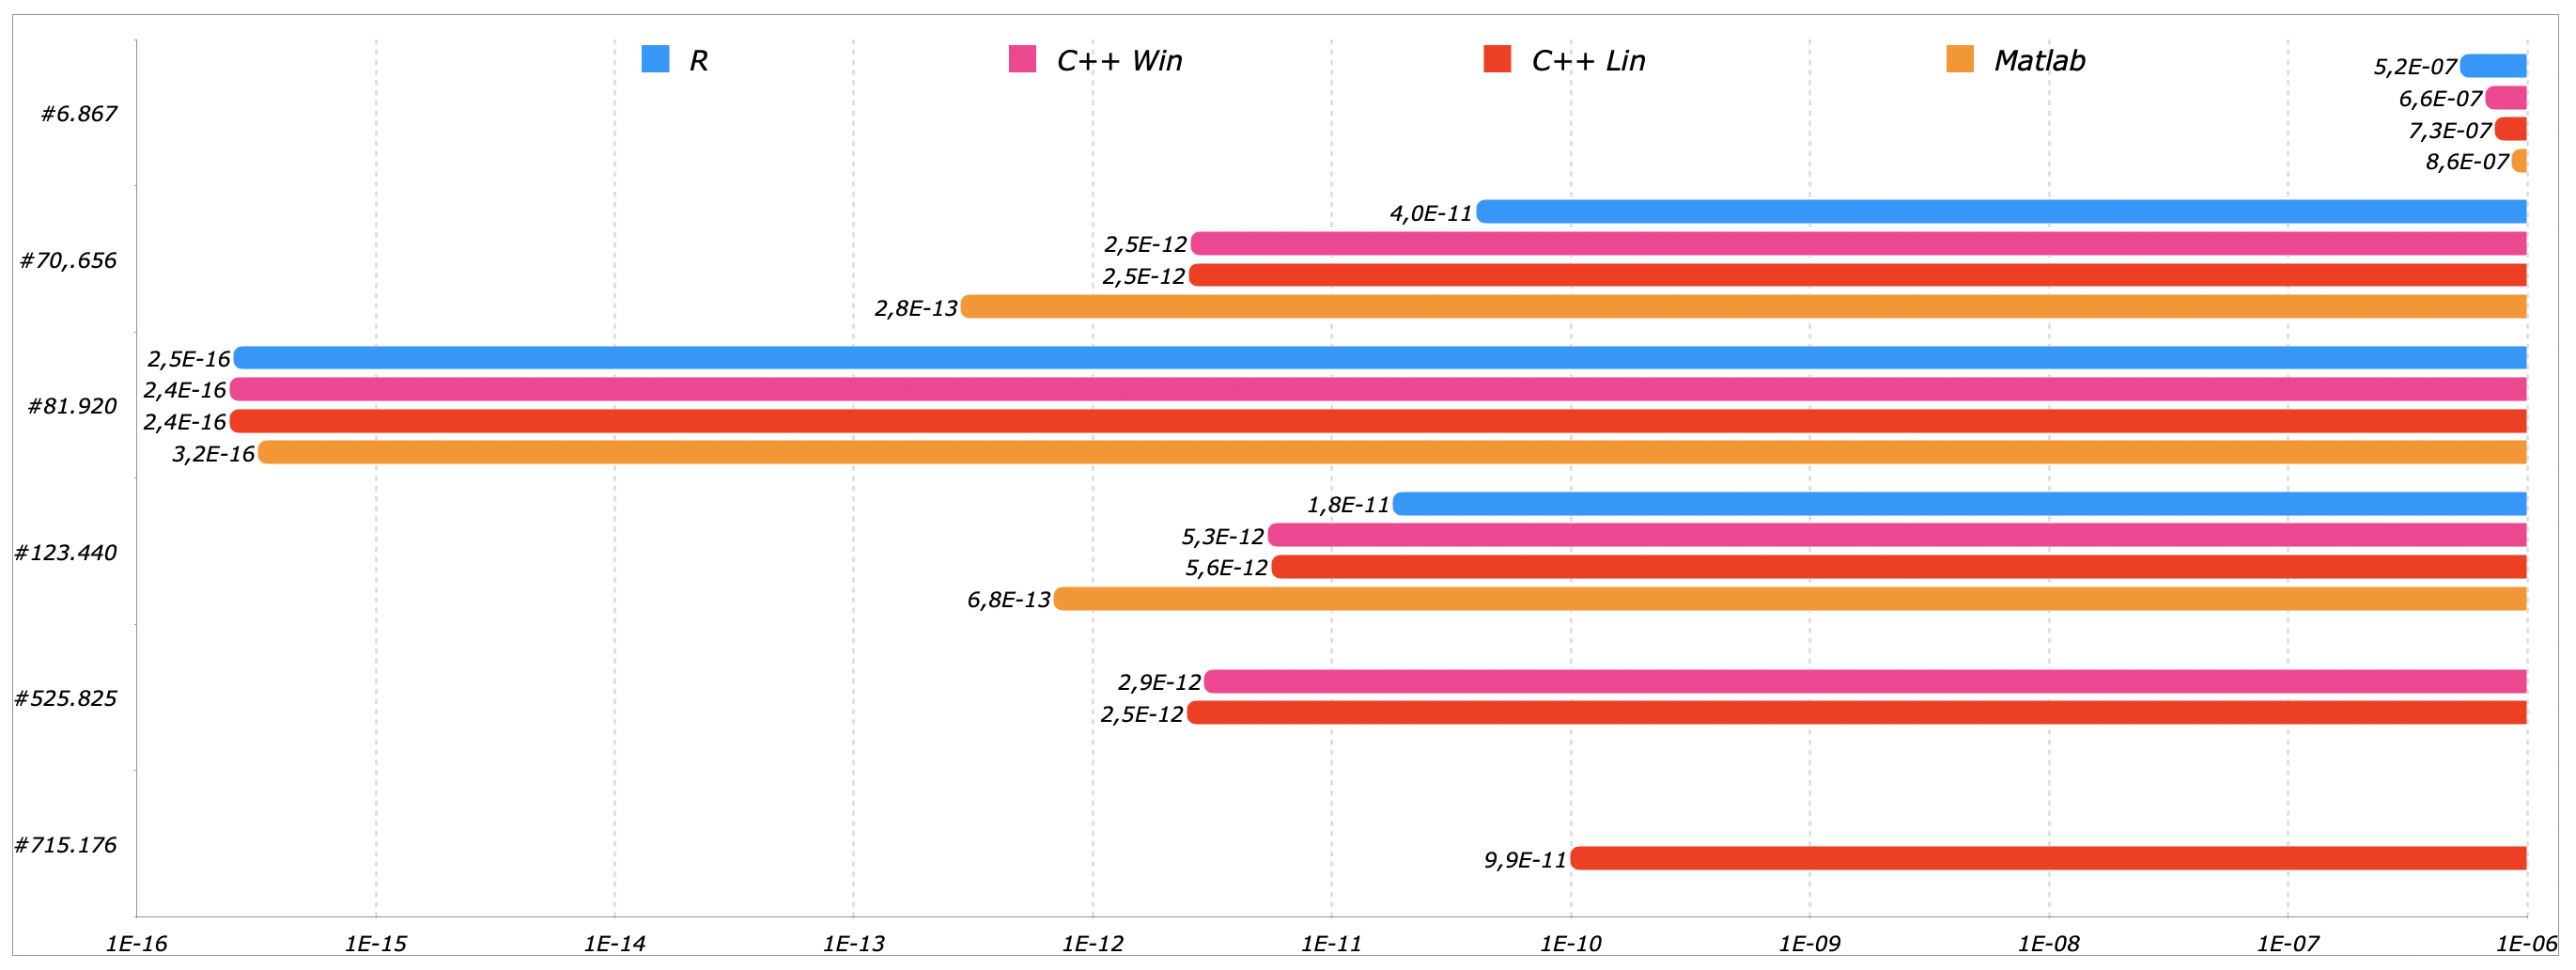
\includegraphics[width=\linewidth]{errore1}
\end{figure}

\begin{figure}[H]
	\centering
	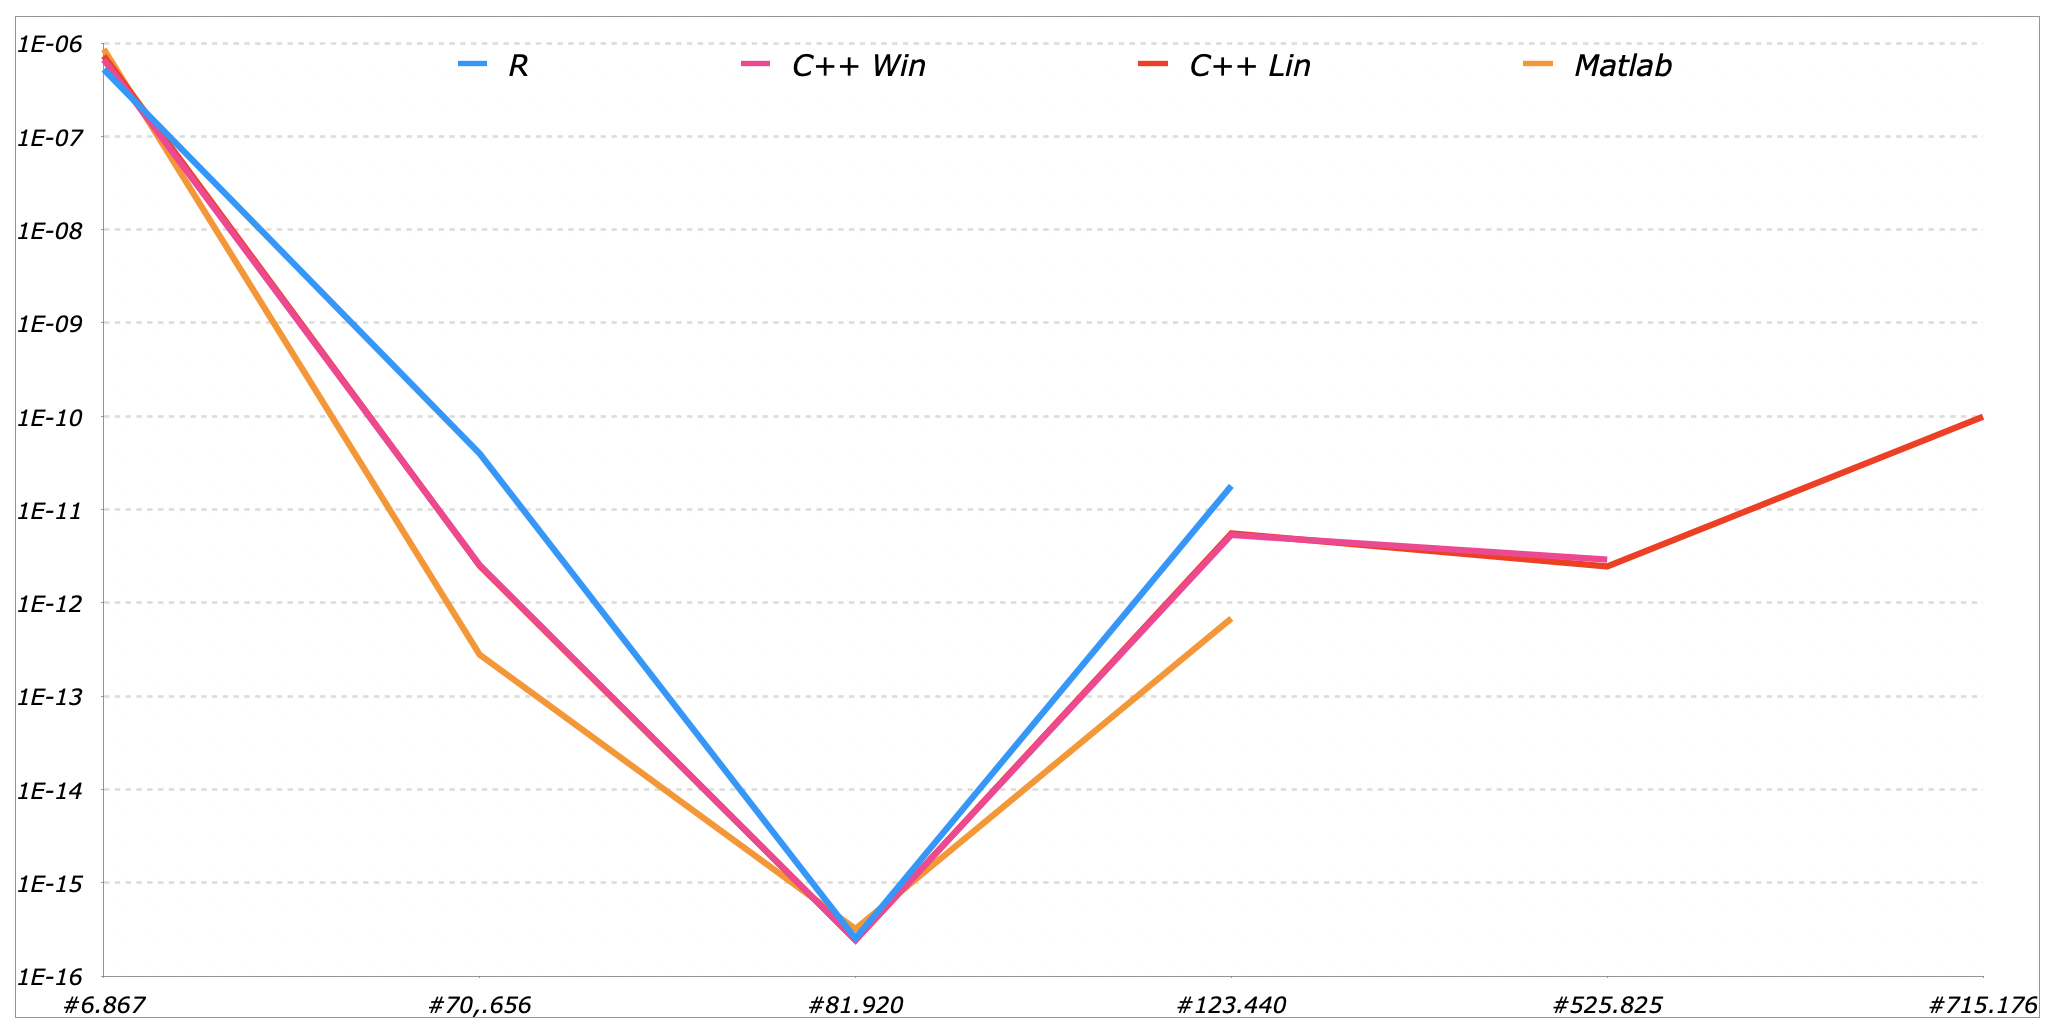
\includegraphics[width=\linewidth]{errore2}
\end{figure}

Si passa ora ad analizzare da un altro punto di vista l'analisi delle diverse elaborazioni. L'errore relativo è un valore che determina con quanta precisione è stata calcolata la soluzione del sistema, in particolare più esso tende a 0 più il calcolo è stato preciso.
Dalle diverse esecuzioni non si può stabilire univocamente quale sia l'ambiente migliore da questo punto di vista, forse Matlab potrebbe esserlo anche se non sempre è il più preciso.\\
Da notare come per la matrice di dimensione 81.920, l'errore relativo sia pressoché il medesimo in tutti i linguaggi.

\subsection{Memoria utilizzata}

\begin{figure}[H]
	\centering
	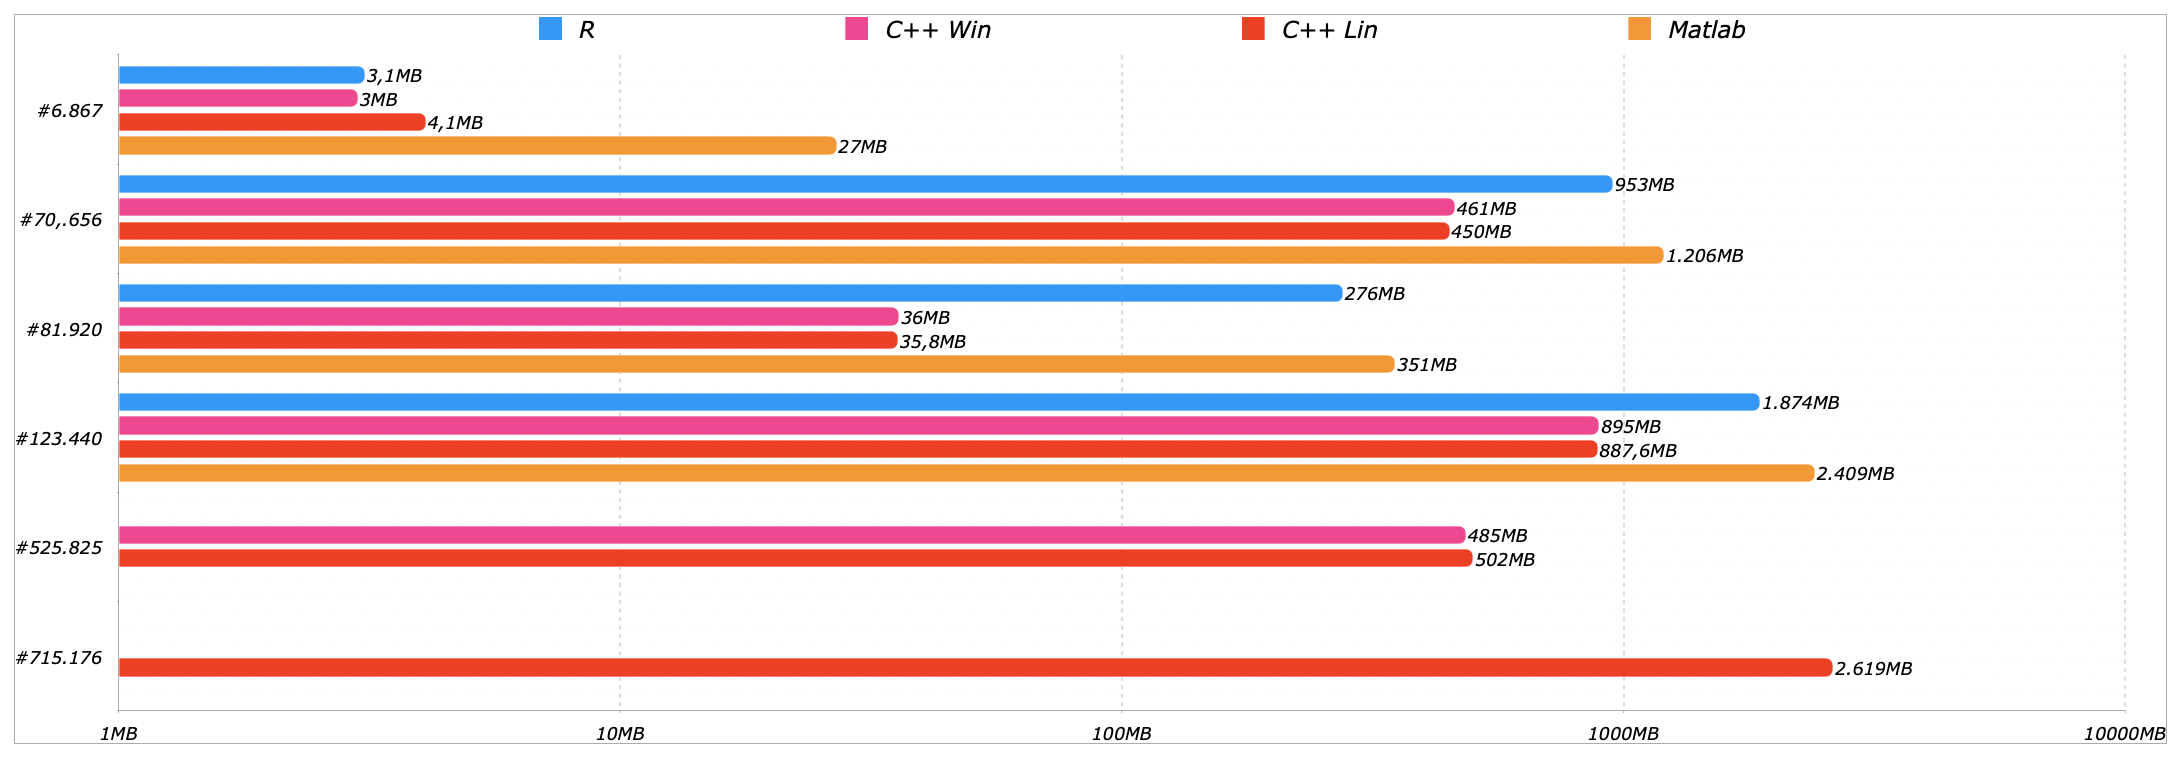
\includegraphics[width=\linewidth]{memoria1}
\end{figure}

\begin{figure}[H]
	\centering
	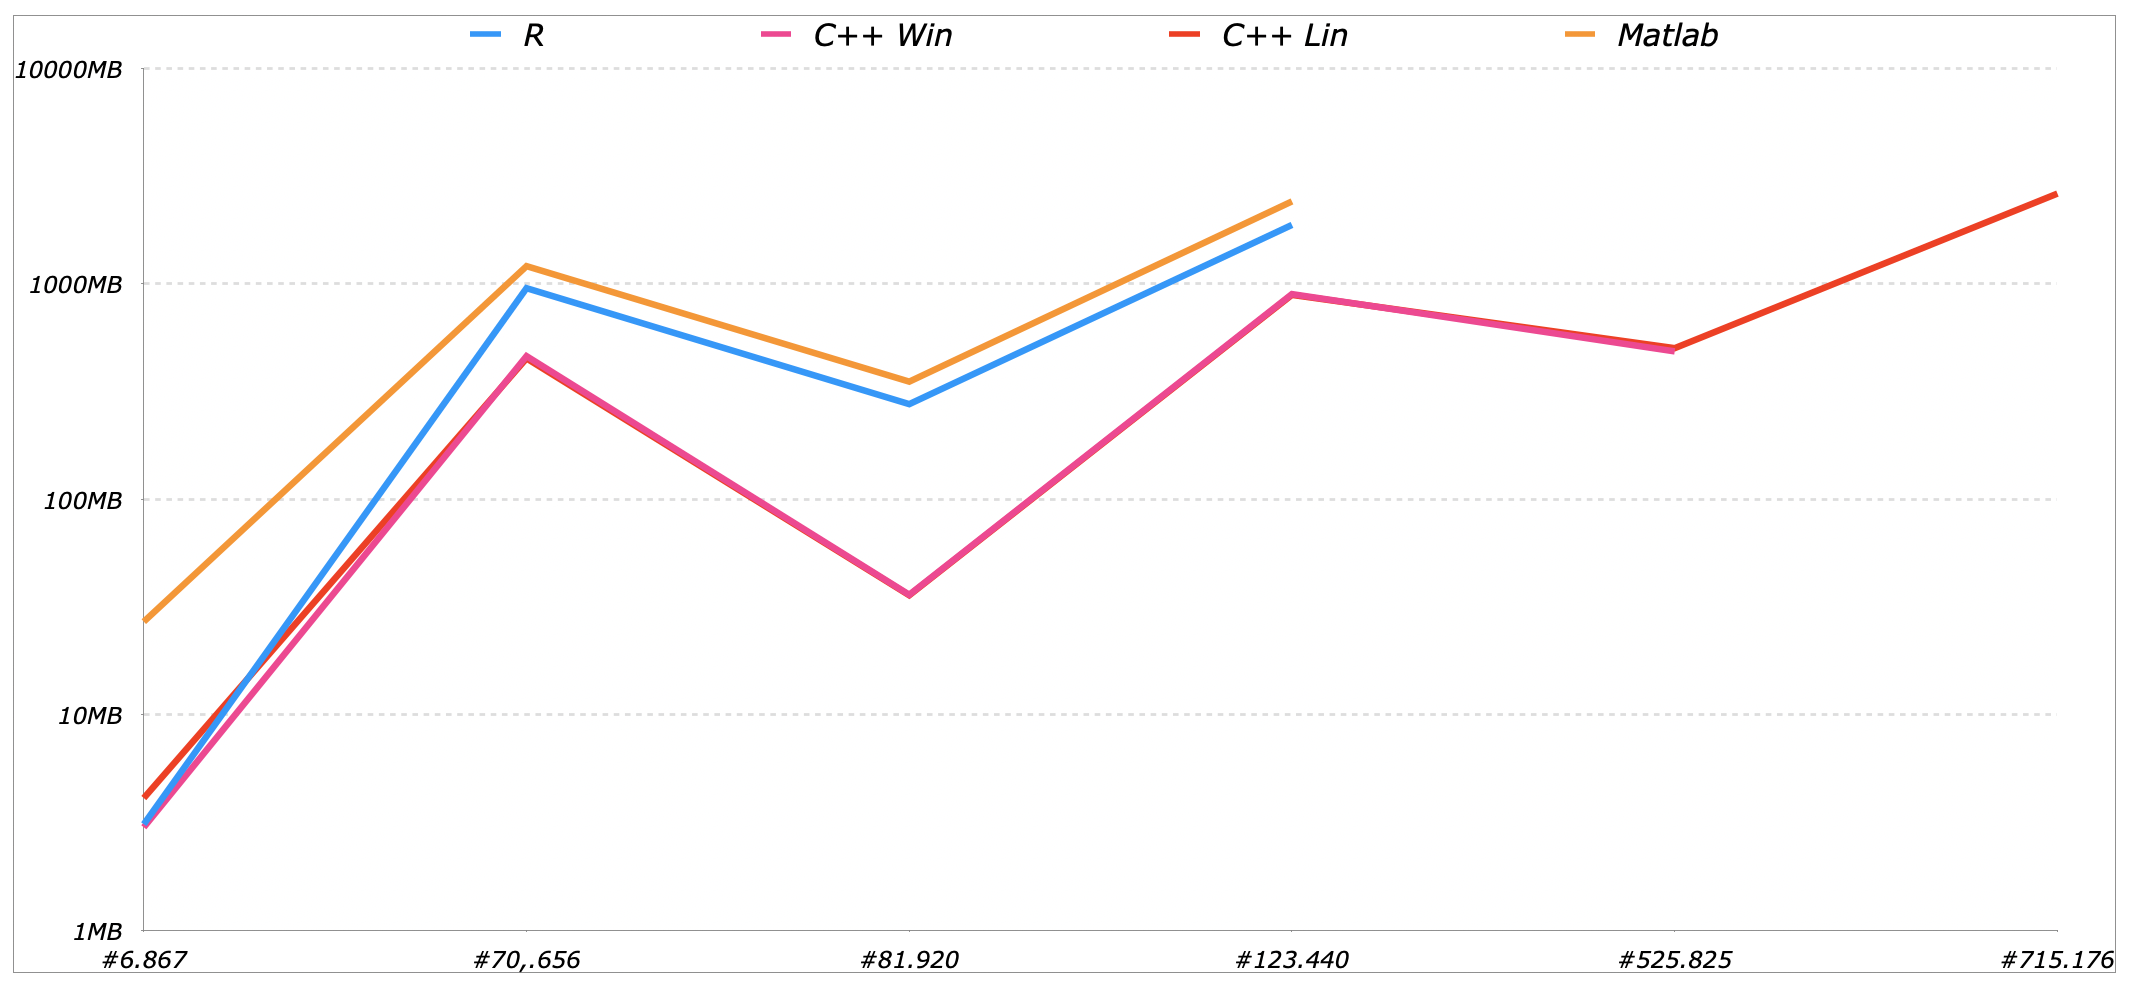
\includegraphics[width=\linewidth]{memoria2}
\end{figure}

Infine vengono riportati i grafici della memoria utilizzata. Questi risultati stravolgono in parte quello acquisito fino ad ora.
Se infatti fino ad adesso Matlab si è rivelato il "migliore", soprattutto per quanto riguarda la velocità di esecuzione, per quanto riguarda la memoria esso è un vero e proprio \textit{memory killer}, utilizza infatti quantitativi di memoria superiori rispetto agli altri, decisamente superiori rispetto alle implementazioni C++, infatti queste ultime riescono a gestire matrici di dimensioni maggiori senza incappare in problemi di \textit{out of memory}.

Curioso notare come la memoria utilizzata da Matlab per la risoluzione di un sistema di dimensione 123.440 è dello stesso ordine di grandezza della memoria utilizzata da C++ per un sistema di 715.176 righe!

\section{Conclusioni}
All'inizio del progetto ci siamo chiesti cosa era meglio tra il software proprietario Matlab oppure un software open source per la risoluzione dei sistemi lineari e anche se era meglio utilizzare tali software in ambiente linux oppure windows. Ecco le risposte:

\begin{enumerate}
\item \textbf{\`E meglio lavorare in ambiente Linux oppure in ambiente Windows?}\\
Come si può evincere dallo studio fatto fin ora, la differenza tra i due ambienti, a parità di software utilizzato, risulta quasi impercettibile. La differenza sostanziale sta nell'uso della memoria.\\
In ambiente Linux, C++ riesce a ottimizzare meglio l'utilizzo della memoria rispetto a Windows, ma questo non comporta in alcun modo differenze sostanziali nelle tempistiche di calcolo.

\item \textbf{\`E meglio affidarsi alla sicurezza di Matlab pagando oppure vale la pena
di avventurarsi nel mondo open source?}\\
Come visto nei grafici presentati in precedenza, Matlab è sempre stato il migliore in termini di tempo e di accuratezza. Purtroppo però non si può dire lo stesso per quanto riguarda l'uso della memoria che, come nel nostro caso, utilizzando calcolatori di fascia media con 8 GB di RAM si incorre nel problema di \textit{out of memory}. In sostanza il vero interrogativo al quale ci siamo sottoposti durante lo studio dei software, è stato "riuscirà a risolvere il sistema lineare o fallirà per mancanza di memoria?". C++ è stato indubbiamente il software che è riuscito a darci più dati su cui lavorare rispetto agli altri, in quanto è stato l'unico che é riuscito a spingersi fino ai sistemi lineari di 715 mila righe e colonne.\\
In conclusione Matlab risulta essere sicuramente il software più prestante in termini di tempo e di errore, mentre C++ è il più prestante in termini di utilizzo della memoria.\\
Sicuramente se non si hanno problemi di utilizzo della memoria, Matlab è la soluzione.
\end{enumerate}
 
\end{document}
%%
%% End of file `elsarticle-template-1-num.tex'.
